\subsection{Modeling Language for System Design}
\label{subsec:aadl-agree}
Figure~\ref{fig:proposed_safety_process} presents our proposed use of a single unified model to support both system design and safety analysis. It describes both system design and safety-relevant information 
that are kept distinguishable and yet are able to interact with each other. The shared model is a living model that captures the current state of the system design as it moves through the development lifecycle, allowing all participants of the \gls{arp}4754A process to be able to communicate and review the system design. Safety related information can be generated directly through automated analysis on the model. This provides the capability to more accurately analyze complex systems. The generated safety information includes counterexamples which show causal failure scenarios and minimal sets of fault combinations that cause the failure condition to occur.

\begin{figure}[t!]
	
	\centering
	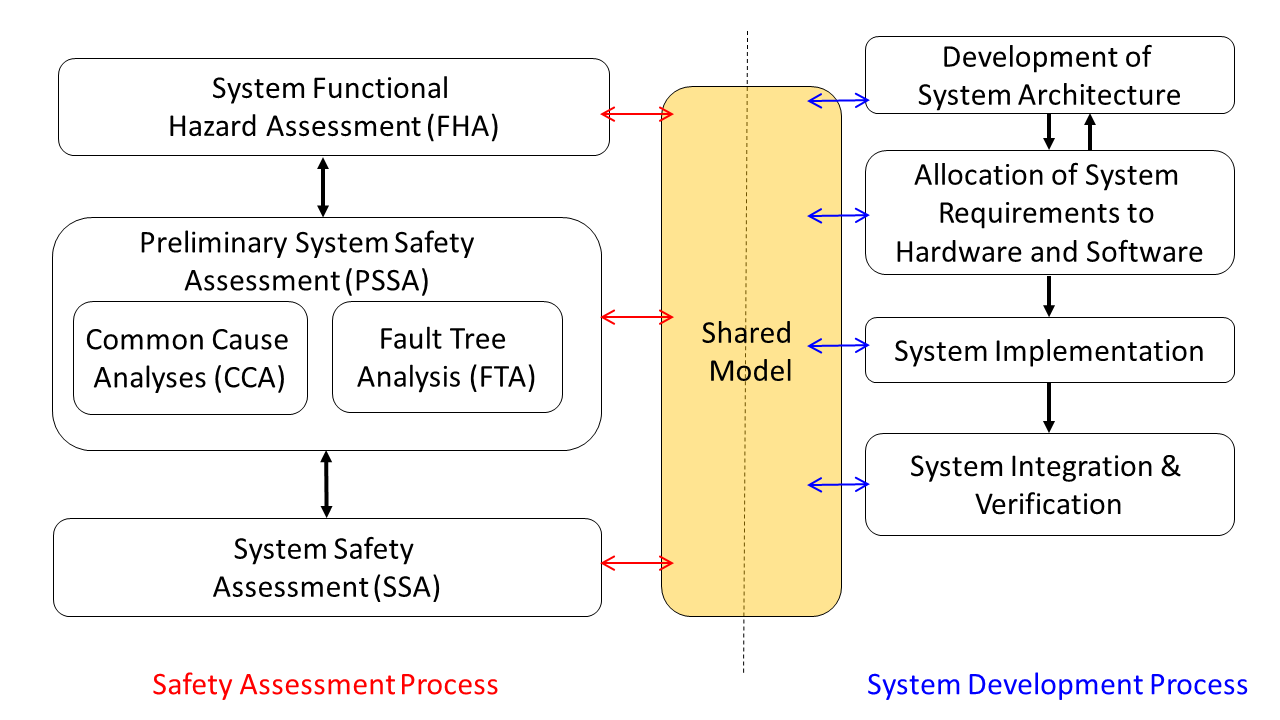
\includegraphics[trim=0 5 0 5,clip,width=0.85\textwidth]{images/process3.png}
	
	\caption{Use of the Shared System/Safety Model in the ARP4754A Safety Assessment Process}
	\label{fig:proposed_safety_process}
\end{figure}

We are using the Architectural Analysis and Design Language (AADL)~\cite{FeilerModelBasedEngineering2012} to construct system architecture models.  \gls{aadl} is an SAE International standard that defines a language and provides a unifying framework for describing the system architecture for ``performance-critical, embedded, real-time systems''~\cite{AADL_Standard}. From its conception, \gls{aadl} has been applied to the design and construction of avionics systems.  
Rather than being merely descriptive, \gls{aadl} models can be made specific enough to support system-level code generation.  Thus, results from analyses conducted, including the new safety analysis proposed here, correspond to the system that will be built from the model.  

An \gls{aadl} model describes a system in terms of a hierarchy of components and their interconnections, where each component can either represent a logical entity (e.g., application software functions, data) or a physical entity (e.g., buses, processors, memory). An \gls{aadl} model can be extended with language annexes to provide a richer set of modeling elements for various system design and analysis needs (e.g., performance-related characteristics, configuration settings, dynamic behaviors). The language definition is sufficiently rigorous to support formal analysis tools that allow for early phase error/fault detection.

The \gls{agree}~\cite{NFM2012:CoGaMiWhLaLu} is a tool for formal analysis of behaviors in \gls{aadl} models.  \gls{agree} is implemented as an \gls{aadl} annex and annotates \gls{aadl} components with formal behavioral contracts. Each component's contracts can include assumptions and guarantees about the component's inputs and outputs respectively, as well as predicates describing how the state of the component evolves over time. \gls{agree} translates an \gls{aadl} model and the behavioral contracts into Lustre~\cite{Halbwachs91:IEEE} and then queries the JKind
model checker~\cite{2017arXiv171201222G} to conduct the back-end analysis. The analysis %is
can be performed compositionally following the architecture hierarchy such that analysis at a higher level is based on the components at the next lower level.  When compared to monolithic analysis (i.e., analysis of the flattened model composed of all components), the compositional approach allows the analysis to scale to much larger systems~\cite{NFM2012:CoGaMiWhLaLu}. 

%In the avionics context, the software functions/applications, the hardware equipment, and the system that is composed of their integration can all be represented as components connected to/composed of/bind to other components in a hierarchical AADL model. AGREE contracts can be used to capture the functional requirements at each level of the hierarchy. Once the model has been reviewed and the requirements captured have been validated, the back-end analysis can be conducted to verify if each level of the model implements its higher level requirements correctly.

%AADL with the AGREE extension serves as a good candidate as the modeling language for describing the system design aspects of a shared system design and safety analysis model. 
%In our prior work~\cite{Stewart17:IMBSA}, we added an initial failure effect modeling capability to the AADL/AGREE language and tool set.  We are continuing this work so that our tools and methodology can be used to satisfy system safety objectives of ARP4754A and ARP4761.  

\begin{comment}
In particular, our goals are to:

\begin{itemize}
	\item Provide a comprehensive, qualitative description of the causal relationship between basic failure events and system level safety requirements.
	\item Provide an accurate, quantitative description of the contribution relationship between failure rates of the fault tree basic events and numerical probability requirements at the system level.
\end{itemize}
\end{comment}
%The remainder of the paper describes our approach towards both of the goals.



